\section{Exception Handling in Threads}\label{sec:ExceptionHandlingInThreads}
When we execute the Java program below, the \lstinline|Error|\index{java.lang!Error} is printed to the console:
\lstinputlisting{coding/errorHandling/TestAbortMain.java}

%\begin{verbatim}
%$ java TestAbortMain.java
%Exception in thread "main" java.lang.Error: Aborted
%	at TestAbortMain.main(TestAbortMain.java:5)
%$ 
%\end{verbatim}

\begin{center}
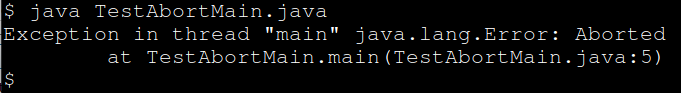
\includegraphics[scale=0.6]{coding/errorHandling/TestAbortMain}
\end{center}

In the sample below, we abort a secondary thread:
\lstinputlisting{coding/errorHandling/TestAbortThread.java}

When executed with contemporary versions of Java, the output will look like the screenshot below; for older versions of Java (before Java~5), there wouldn't be shown any output from the thread at all:






\chapter*{Road Work ahead!}








%\begin{verbatim}
%$ java TestAbortRun.java
%Exception in thread "Thread-0" java.lang.Error: run() aborted!
%	at TestAbortRun.run(TestAbortRun.java:5)
%	at java.base/java.lang.Thread.run(Thread.java:1474)
%Exception in thread "main" java.lang.Error: main() aborted!
%	at TestAbortRun.main(TestAbortRun.java:20)
%$ 
%\end{verbatim}

\begin{center}
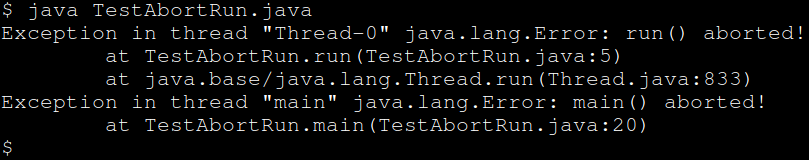
\includegraphics[scale=0.5]{coding/errorHandling/TestAbortRun}
\end{center}

\chapter*{Road Work done!}


This behaviour can be sufficient for a tool\index{product type!tool} (see chapter \tqref{sec:Tool} on page \pageref{sec:Tool}) or a script (chapter \tqref{sec:ScriptInJava} on page \pageref{sec:ScriptInJava}), but it is not feasible for a standalone application\index{product type!standalone application} (chapter \tqref{sec:StandaloneApplication} on page \pageref{sec:StandaloneApplication}) and not for a feature library\index{product type!feature library} (chapter \tqref{sec:FeatureLibrary} on page \pageref{sec:FeatureLibrary}).

A function library\index{product type!function library} (chapter \tqref{sec:FunctionLibrary} on page \pageref{sec:FunctionLibrary}) usually relies for the reporting of error conditions on the caller of a method\index{method}, while server-based applications\index{product type!server-based application} (chapter \tqref{sec:ServerbasedApplication} on page \pageref{sec:ServerbasedApplication}) and extensions\index{product type!extension} (chapter \tqref{sec:Extension} page \pageref{sec:Extension}) use the facilities provided by the host applications for this purpose.

For both a standalone application\index{product type!standalone application} and for a feature library\index{product type!feature library}, you want that error conditions will be tracked somehow\footnote{usually this means logging - see chapter \tqfullvref{sec:Logging}}, under all circumstances, and from all threads – because no error may go unnoticed, as required in the \ngref, bullet point~\ref{lst:ZoP:ErrorsMayNeverBeSwallowed}.

The payload of a thread\index{thread} is an implementation of the method \lstinline|run()|\index{java.lang!Runnable!run()} \autocite{ORACLE_DOC_RUNNABLE:run} from the interface \lstinline|java.lang.Runnable|\index{java.lang!Runnable} \autocite{ORACLE_DOC_RUNNABLE_INTERFACE}. 

You find quite often code in such implementations that follows the pattern shown below. Sometimes a \lstinline|catch|\index{try!catch} clauses for \lstinline|java.lang.RuntimeException|\index{java.lang!RuntimeException}, or even \lstinline|java.lang.Throwable|\index{java.lang!Throwable} are used, instead of one for \lstinline|java.lang.Exception|\index{java.lang!Exception}.

\keeplisting{7}
\index{java.lang!Exception}
\begin{lstlisting}
// DISCOURAGED!!
public final void run()
{
    try
    {
        // Do whatever this thread must do …
    }
    catch( final Exception e ) // DON'T CATCH EXCEPTION!!!
    {
        m_Logger.error( "No matter what went wrong, but I will log the exception", e );
    }
} 
\end{lstlisting}

This is a very bad excuse for a \lstinline|catch|\index{try!catch} clause for \lstinline|Exception|\index{java.lang!Exception}, \lstinline|RuntimeException|\index{java.lang!RuntimeException} or \lstinline|Throwable|\index{java.lang!Throwable}!

This is so bad because this code pattern absolves the programmer of the duty to properly handle any exceptions\index{exception} thrown within the \lstinline|try|\index{try} block individually – with a \lstinline|catch|\index{try!catch} clause for \lstinline|java.lang.Exception|\index{java.lang!Exception} even including the checked\index{exception!checked exception} ones – because the \lstinline|catch|\index{try!catch} block at the end will take care of all exceptions.

The best practice here is to set the \bdq{Uncaught Exception Handler}\index{java.lang!Thread.UncaughtExceptionHandler} \autocite{ORACLE_DOC_UNCAUGHTEXCEPTIONHANDLER_INTERFACE} for the thread\index{thread}, either through the \lstinline|ThreadFactory|\index{java.util.concurrent!ThreadFactory} \autocite{ORACLE_DOC_THREADFACTORY_INTERFACE}, through the \lstinline|ThreadGroup|\index{java.lang!ThreadGroup} \autocite{ORACLE_DOC_THREADGROUP_CLASS} or individually. 

\keeplisting{1}
\lstinline|java.lang.Thread.UncaughtExceptionHandler|\index{java.lang!Thread.UncaughtExceptionHandler} is a functional interface\index{interface!functional interface} that can be easily implemented as a method\index{method} like this:
\begin{lstlisting}[caption=UncaughtExceptionHandler as Method]
private static final void uncaughtExceptionHandler( final Thread t, final Throwable e )
{
    final var throwableType = e instanceof Error ? "error" : "exception";
    final var message = """
````````Thread "%s" was aborted with an %s!\
````````""".formatted( t.getName(), throwableType ) 
    m_Logger.atFatal()
        .withThrowable( e )
        .log( message );    
}   //  uncaughtExceptionHandler()
\end{lstlisting}
When you need to set the uncaught exception handler\index{java.lang!Thread.UncaughtExceptionHandler}, you refer to that method with a method reference: \lstinline|<Class>::uncaughtExceptionHandler|.

Of course it can be implemented as a class as well:
\begin{lstlisting}[caption=UncaughtExceptionHandler as Class]
/**
 *  <p>{@summary An implementation for
 *  {@link UncaughtExceptionHandler}.}</p>
 */
public final class UncaughtExceptionHandlerImpl implements UncaughtExceptionHandler
{
        /*------------------------*\
    ====** Static Initialisations **======================================
        \*------------------------*/
    /**
     *  <p>{@summary The instance of this class.}</p>
     */
    public static final UncaughtExceptionHandler INSTANCE = new UncaughtExceptionHandlerImpl();

    /**
     *  <p>{@summary The logger that is used to log the exceptions.}</p>
     */
    private static final Logger m_Logger = getLogger( UncaughtExceptionHandler.class.getName() );

        /*--------------*\
    ====** Constructors **================================================
        \*--------------*/
    /**
     *  <p>{@constructor}}</p>
     */
    public UncaughtExceptionHandlerImpl() { /* Just exists */ }

        /*---------*\
    ====** Methods **=====================================================
        \*---------*/
    /**
     *  {@inheritDoc}
     */
    @Override
    public final void uncaughtException( final Thread t, final Throwable e )
    {
        final var throwableType = e instanceof Error ? "error" : "exception";
        final var message = """
````````````Thread "%s" was aborted with an %s!\
````````````""".formatted( t.getName(), throwableType ); 
        m_Logger.atFatal()
            .withThrowable( e )
            .log( message );    
    }   //  uncaughtException()
}
//  class UncaughtExceptionHandlerImpl
\end{lstlisting}

\keeplisting{1}
Or as an anonymous class\index{class!anonymous class}
\begin{lstlisting}[caption=UncaughtExceptionHandler as Anonyomous Class]
private static final UncaughtExceptionHandler = m_UncaughtExceptionHandler = new Thread.UncaughtExceptionHandler()
{
    /**
     *  {@inheritDoc}
     */
    @Override
    public final void uncaughtException( final Thread t, final Throwable e )
    {
        final var throwableType = e instanceof Error ? "error" : "exception";
        final var message = """
````````````Thread "%s" was aborted with an %s!\
````````````""".formatted( t.getName(), throwableType ); 
        m_Logger.atFatal()
            .withThrowable( e )
            .log( message );    
    }   //  uncaughtException()
};
\end{lstlisting}

\keeplisting{3}
Setting the uncaught exception handler\index{java.lang!Thread.UncaughtExceptionHandler} for an individual thread\index{thread} looks like this:
\begin{lstlisting}
Thread.ofPlatform()
    .group( threadGroup )
    .uncaughtExceptionHandler( this::uncaughtExceptionHandler )
    .start( () -> {…} );
\end{lstlisting}
Here the method \lstinline|uncaughtExceptionHandler()|is not static; that can be usefull when the failure message should depend on the instance.

\keeplisting{3}
For a thread pool\index{thread pool}, the code would be similar to this:
\begin{lstlisting}
final var factory = Thread.ofPlatform()
    .group( threadGroup )
    .uncaughtExceptionHandler( this::uncaughtExceptionHandler )
    .factory();
final var threadPool = Executors.newCachedThreadPool( factory );
\end{lstlisting}

If the uncaught exception handler\index{java.lang!Thread.UncaughtExceptionHandler} is provided by the \lstinline|ThreadGroup|\index{java.lang!ThreadGroup} instance, the call to \lstinline|Builder::uncaughtExceptionHandler|\index{java.lang!Thread.Builder!uncaughtExceptionHandler()} should be omitted; otherwise it overwrites the setting from the group.

A thread group is supported only by platform threads\index{thread!platform thread}, not by virtual threads\index{thread!virtual thread}. Additionally, the \lstinline|ThreadGroup|\index{java.lang!ThreadGroup} implementation provided by the \Java Runtime Library does not allow to set a custom uncaught exception handler. In chapter \tqref{sec:ThreadGroup} on page \pageref{sec:ThreadGroup} I show an implementation of \lstinline|ThreadGroup|\index{java.lang!ThreadGroup} that got that feature added.

Through the static method \lstinline|Thread::setDefaultUncaughtExceptionHandler|\index{java.lang!Thread!setDefaultUncaughtExceptionHandler()} \autocite{ORACLE_DOC_THREAD:setDefaultUncaughtExceptionHandler} you can even define a default handler that is used by all threads that does not specify an individual one, as shown in chapter \tqfullvref{sec:MethodMain}.

Usually a thread should use the \lstinline|UncaughtExceptionHandler|\index{java.lang!Thread.UncaughtExceptionHandler} that is assigned to it on creation. But if your method\index{method} requires a special treatment for an uncaught exception when executed within a thread from a thread pool, the method\index{method} can set an individual uncaught exception handler\index{java.lang!Thread.UncaughtExceptionHandler} as shown in the code sample below.

\index{java.lang!Runnable!run()}\index{java.lang!Thread!currentThread()}\index{java.lang!Thread!getDefaultUncaughtExceptionHandler()}\index{java.lang!Thread!setDefaultUncaughtExceptionHandler()}\index{java.lang!Thread.UncaughtExceptionHandler}
\begin{lstlisting}
public final void run()
{
    final var currentThread = Thread.currentThread();
    final var uncaughtExceptionHandler = currentThread.getUncaughtExceptionHandler();
    currentThread.setUncaughtExceptionHandler( (t,e) ->
    {
        /*
         * The special exception treatment goes here …
         *

        //---* Finally log the exception *--------------------------------
        m_Logger.fatal( () -> """
````````````````Thread "%s" was aborted with an exception!\
````````````````""".formatted( t.getName() ), e );
    } );
 
    try
    {
        /*
         * Do whatever this thread must do …
         */
    }
    finally
    {
        //---* Reset the uncaught exception handler *---------------------
        currentThread.setUncaughtExceptionHandler( uncaughtExceptionHandler );
    }
}   //  run()
\end{lstlisting}

That \bdq{special treatment} could be an individual message, but also that you want to log the issue in a different manner or to another location.

If your code changes the uncaught exception handler\index{java.lang!Thread.UncaughtExceptionHandler} of the thread that executes that code, it must restore the handler before it terminates, because threads from a thread pool are reused with different payloads (during their lifetime, they execute the \lstinline|run()|\index{java.lang!Runnable!run()} method from different instances of \lstinline|Runnable|\index{java.lang!Runnable} implementations). Although virtual threads\index{thread!virtual thread} are not reused\footnote{At least not if you follow the recommendations given in JEP~444 \autocite{JEP444:Pooling}.}, you should restore the uncaught exception handler\index{java.lang!Thread.UncaughtExceptionHandler} even when \lstinline|Thread::isVirtual|\index{java.lang!Thread!isVirtual()} \autocite{ORACLE_DOC_THREAD:isVirtual} returns \lstinline|true| for the current thread\index{thread}.

%==============================================================================
% End of file!!
%==============================================================================
